%
%  Scott Percic
%
\documentclass[12pt,fullpage]{article}
\usepackage{fullpage}
\usepackage{psfrag}                                          % LaTeX graphics tool
\usepackage{pslatex}                                         % avoids the default cmr font
\usepackage{graphicx}                                        % graphics package 
\usepackage{epsfig}                                          % figures
\usepackage{hyperref}
\usepackage{color}

\begin{document}

\noindent
{\bf Log normal distribution} (from \color{blue}\url{http://www.math.wm.edu/~leemis/chart/UDR/UDR.html}\color{black})

\noindent
The shorthand $X \sim {\rm log\  normal}(\alpha,\, \beta)$ is used to indicate that the
random variable $X$ has the log normal distribution with parameters $\alpha$ and $\beta$.
A log normal random variable $X$ with parameters $\alpha$ and $\beta$ has probability density function 
$$
f(x) = \frac{1}{\kern 0.08 em x \kern 0.08 em \beta \sqrt{2\pi}} \kern 0.08 em e ^ {-\frac{1} {2}(\ln (x/ \alpha) / \beta) ^ {2}} \qquad \qquad x > 0
$$
for $\alpha$ and $\beta > 0$.  
The log normal distribution can be used to model the lifetime of an object, the weight of a person, or a service time.
The central limit theorem indicates that the log normal distribution is
useful for modeling random variables that can be thought of as a 
product of several independent random variables.
The probability density function with three different parameter settings is illustrated below.
{\begin{figure}[h!]
\begin{center}
\psfrag{lab1}{$\alpha \kern -0.08 em = \kern -0.08 em  1,\, \beta \kern -0.08 em  = \kern -0.08 em  1$}
\psfrag{lab2}{$\alpha \kern -0.08 em  = \kern -0.08 em  1,\, \beta \kern -0.08 em  = \kern -0.08 em  2$}
\psfrag{lab3}{$\alpha \kern -0.08 em  = \kern -0.08 em  5,\, \beta \kern -0.08 em  = \kern -0.08 em  0.5$}
\psfrag{labx}{$x$}
\psfrag{labf}{$f(x)$}
\includegraphics[width=3.2in]{LognormalPlot.ps}
\end{center}
\end{figure}}\\
The cumulative distribution function on the support of $X$ is
$$
F(x) = P(X \le x) = \frac{1}{2} + \frac{1}{2}\,
{{\rm erf} \left({\frac {\sqrt {2} \left( \ln  \left( x \right) - \alpha  \right) }{2\beta }}\right)}
 \qquad \qquad  x > 0, 
$$
where
$$
{\rm erf}(x) = \frac{2}{\sqrt{\pi}} \int_{0} ^ {x} e ^ {-t ^ {2}} \, dt.
$$
The survivor function on the support of $X$ is
$$
S(x) = P(X \ge x) = \frac{1} {2} - \frac{1} {2}\,
{{\rm erf}\left({\frac {\sqrt {2} \left( \ln  \left( x \right) - \alpha  \right) }{2\beta }}\right)}\qquad \qquad
x > 0.
$$
The hazard function on the support of $X$ is
$$
h(x) = \frac{f(x)}{S(x)} = -\sqrt {2}{e^{- \left( \ln  \left( x \right) -
\alpha  \right) ^ {2}/ {2\beta }^{2}}}{\frac {1}{\sqrt {\pi }}}\kern 0.08 em {x}^{-1
}{\beta }^{-1} \left( -1+
{{\rm erf}\left({\frac {\sqrt {2} \left( \ln  \left( x \right) -\alpha  \right) }{2\beta }}\right)}
 \right) ^{-1}
 \qquad x > 0.
$$
The cumulative hazard function on the support of $X$ is
$$
H(x) = - \ln S(x) =\ln  \left( 2 \right) +i \kern 0.08 em \pi -\ln  \left( -1+
{{\rm erf}\left({\frac {\sqrt {2} \left( \ln  \left( x \right) -\alpha  \right) }{2\beta }}\right)}
 \right) \qquad \qquad x > 0.
$$
The inverse distribution function, moment generating function, and characteristic function of $X$ are mathematically intractable.\\
\\
The median of $X$ is $\alpha.$\\
\\
The population mean, variance, skewness, and kurtosis of $X$ are
$$
E[X] = \alpha e^{\beta^2/2} \qquad \qquad 
V[X] = \alpha^2 e^{\beta^2} (e^{\beta^2} - 1)
$$
\\
\vspace{-.35in}
$$
E\left[ \left( \frac{X - \mu}{\sigma} \right) ^ {\kern -0.08 em 3} \right] = (e^{\beta^2} + 2)(e^{\beta^2} - 1)^{1/2} \qquad \qquad
E\left[ \left( \frac{X - \mu}{\sigma} \right) ^ {\kern -0.08 em 4} \right] = e^{4 \beta^2} + 2 e^{3 \beta^2} + 3 e^{2 \beta^2} - 3
$$
\vspace{0.1in}

\noindent
{\bf APPL verification:}
The APPL statements
\begin{verbatim}
assume(alpha > 0);
assume(beta > 0);
X := [[x-> (1/(x*beta*sqrt(2*Pi)))*exp((-1/2)*(ln(x/alpha)/beta)^2)],
     [0,infinity],["Continuous","PDF"]];
CDF(X);
SF(X);
HF(X);
CHF(X);
Mean(X);
Variance(X);
Skewness(X);
Kurtosis(X);
\end{verbatim}
verify the cumulative distribution function, survivor function, hazard function, cumulative hazard function, population mean, variance, skewness, and kurtosis.
\end{document}
